\section{Стабилизация положения равновесия модельного уравнения} \label{p22}

Рассмотрим решение задачи стабилизации в области 
$G = {(x, \dot x) \in R^4 : \|x\|<\epsilon, \|\dot x\|<\epsilon, \epsilon=const>0}$
с помощью непрерывного управления вида

$$U^{(1)}(x, \dot x) = B(\dot x + p(x))$$ \label{2.3'}     

где $B \in R^{2 \times 2}$ есть матрица коэффициентов усиления сигналов, подлежащая определению.
Возьмем для системы (2.2) вектор-функцию Ляпунова $V = (V^1, V^2)^{'}$  с коэффициентами вида $V^1 = \|p(x)\|, V^2 = \sqrt{(\dot x + p(x))^{'} A^{(1)}(t, x)(\dot x + p(x))}$.

Вычисляя производную по времени вектор-функции Ляпунова $V$ в силу системы (2.1), получим следующие оценки:
$$ \dot V^1 \le -mu_1 V^1 + \frac{m_1}{\lambda_1}, \dot V^2 le m_2 V^1 - \mu_2 V^2 + m_3 (V^1)^2 + m_4 (V^2)^2 + m_5 V^1 V^2, $$

где положительные постоянные $\mu_1, \mu_2, \lambda_1, m_i (i=1,2,...,5)$ определяются из следующих условий:

$$\lambda_1^2 = \frac{I_1 + m_2 l_1^2 + I_2 - \sqrt{(I_1 + m_2 l_1^2 - I_2)^2} + 4(m_2 l_1 l_{g_2})^2}{2}$$

$$\lambda_2^2 = \frac{I_1 + m_2 l_1^2 + I_2 + \sqrt{(I_1 + m_2 l_1^2 - I_2)^2} + 4(m_2 l_1 l_{g_2})^2}{2}$$

$\mu_1 =\frac12 \cos(\frac{\epsilon}{2}), m_1 = \frac12, m_2 = \max \frac{\lambda_2^2 + 2 \sqrt{\lambda_{max} [(D-F)^{'} (D-F)]}}{2 \lambda_1}, m_3 = \frac{m_2 l_1 l_{g_2}}{\lambda_1}, m_4 = \frac{2 m_2 l_1 l_{g_2}}{\lambda_1}, m_5 = \frac{3 m_2 l_1 l_{g_2}}{\lambda_1}, \mu_2 = \frac{-\lambda_2^2 - 4 g_1 m_2 l_q l_{g_2} - \lambda_{max} (B + B^{'})}{2 \lambda_2}$

Здесь $\lambda_max$ есть максимальное собственное значение соответствующей матрицы. 
Тогда для системы (2.1) можно построить следующую систему сравнения:

\begin{equation}\label{2.4'}
\dot u^1 = - \mu_1 u^1 + \frac{m_1}{\lambda_1} u^2, \dot u^2 = m_2 u^1 - \mu_2 u^2 + m_3 (u^1)^2 + m_4(u^2)^2 + m_5 u^1 u^2
\end{equation}

Согласно теореме сравнения об асимптотической устойчивости [5] из свойства асимптотической устойчивости нулевого решения системы сравнения (2.4) следует свойство равномерной асимптотической устойчивости нулевого решения системы (2.2). Получим условие асимптотической устойчивости нулевого решения системы (2.4) с областью притяжения $ {(u^1, u^2) \in R^2 : 0 \le u^1 \le \delta_1 = const>0, 0 \le u^2 \le \delta_2 = const>0} $ . Пусть найдется такое число $\gamma>0$, что выполняются соотношения:

\begin{equation}\label{2.5'}
\gamma = \frac{\delta_2 m_1}{\delta_1 \lambda_1 \mu_1}, \mu_2 > \frac{m_1}{\gamma \lambda_1 \mu_1} (m_2 + \delta_1 m_3) + m_4 \delta_2 + m_5 \delta_1
\end{equation}

Тогда можно показать, что функция $\widetilde{u}(t) = \max{(u^1(t), \delta_1 u^2(t)/ \delta_2)}$ будет монотонно стремиться к нулю при $t \to \infty$, и, значит, нулевое решение системы сравнения (2.4) будет асимптотически устойчиво.
При невозможности практической реализации программного управления стабилизацию программного движения можно осуществить при помощи разрывного управления вида

\begin{equation} \label{2.6'}
U^{(1)}(x, \dot x) = B \ sign(\dot x + p(x))
\end{equation}

Численное моделирование движения манипулятора при действии управлений (2.3) и (2.6) проводилось при следующих значениях параметров манипулятора и программной траектории:
$$ m_1 = 0,5 \text{кг}, m_2 = 0,3 \text{кг}, l_1 = 0,5 \text{м}, l_2 = 0,5 \text{м }, l_{g_1} = 0,25 \text{ м},  l_{g_2} = 0,3 м, I_1 = 0,01 \text{ кг} \cdot \text{м\textsuperscript{2}}, \\ I_2 = 0,006 \text{ кг} \cdot \text{м\textsuperscript{2}}, q_1^0(t) = \sin(0,5t), q_1^0(t) = \cos(0,5t) + \pi/2$$
На рисунках 2 и 3 представлены результаты моделирования при управлениях (2.3) и (2.6) соответственно. 

\begin{figure}[h]
	\centering
	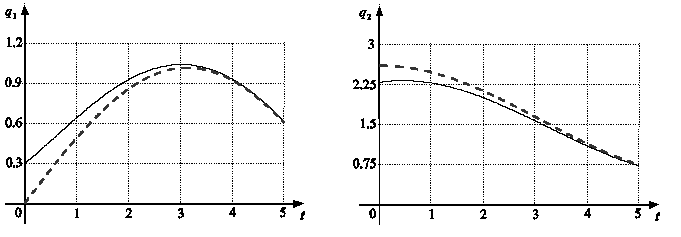
\includegraphics{model1}
	\caption{Результаты моделирования при управлении (2.3)}
	\label{fig:manip2}
\end{figure}

\begin{figure}[h]
	\centering
	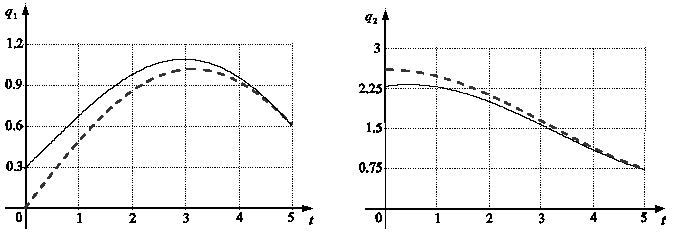
\includegraphics{model2}
	\caption{Результаты моделирования при управлении (2.6)}
	\label{fig:manip3}
\end{figure}
